% -*- TeX-master: "sbml-level-2-version-3"; fill-column: 66 -*-
% $Id$
% $Source$
% ----------------------------------------------------------------

\section{The Systems Biology Ontology and the \token{sboTerm} field}
\label{sec:sboTerm}

The values of \token{id} fields on SBML components allow the
components to be cross-referenced within a model. The values of
\token{name} fields on SBML components provide meaningful labels
suitable for display to humans (Section~\ref{sec:idnameattribs}).
The specific identifiers and labels used in a model necessarily
must be unrestricted by SBML, so that software and users are free
to pick whatever they need.  However, this freedom makes it more
difficult for software tools to determine, without additional
human intervention, the semantics of models more precisely than
the semantics provided by the SBML structures defined in other
sections of this document. For example, there is nothing inherent
in a parameter with identifier ``\token{k}'' that would indicate
to a software tool it is a first-order rate constant (if that's
what ``\token{k}'' happened to be in some given model).  An
advanced software tool \emph{might} be able to deduce the
semantics of some model components by detailed analysis of the
kinetic rate expressions and other parts of the model, but this
quickly becomes infeasible for any but the simplest of models.

An approach to solving this problem is to associate model
components with terms from regulated, controlled vocabularies
(CVs).  This is the purpose of the optional \token{sboTerm} field
provided on the SBML classes \sboelements.  The \token{sboTerm}
field always refers to terms belonging to the Systems Biology Ontology
(SBO, \sboref). In this section, we discuss the \token{sboTerm} field, SBO,
the motivations and theory behind their introduction, and
guidelines for their use.

SBO is not part of SBML; it is being developed separately, to
allow the modeling community to evolve the ontology independently
of SBML.  However, the terms in the ontology are being designed
with SBML components in mind, and are classified into subsets that
can be related one-to-one with SBML components such as reaction
rate expressions, parameters, and a few others.


\subsection{Principles}
\label{sec:sbo-principles}

Labeling model components with terms from shared controlled
vocabularies allows a software tool to identify each component using
identifiers that are not tool-specific.  An example of where this
is useful is the desire by many software developers to provide
users with meaningful names for reaction rate equations.  Software
tools with model editing interfaces frequently provide these names
in menus or lists of choices for users.  However, without a
standardized set of names or identifiers shared between
developers, a given software package cannot reliably interpret the
names or identifiers of reactions in models written by other
tools.

The first solution that might come to mind is to stipulate that
certain common reactions always have the same name (\eg
``Michaelis-Menten''), but this is simply impossible to do: not
only do humans often disagree on the names themselves, but it
would not allow for correction of errors or updates to the list of
predefined names except by issuing new revisions of the SBML
specification---to say nothing of many other limitations with this
approach.  Moreover, the parameters and variables that appear in
rate expressions also need to be identified in a way that software
tools can interpret mechanically, implying that the names of these
entities would also need to be regulated.

The Systems Biology Ontology (SBO) provides vocabularies for
identifying common reaction rate expressions, common
reactant/product/modifier roles in reactions, common parameter
types and their roles in rate expressions, common modeling
frameworks (e.g., ``continuous'', ``discrete'', etc.), but also common types of species and reactions.  The
relationship implied by an \token{sboTerm} value on an SBML model
component is ``is a'': the thing defined by that SBML component
``is an'' instance of the thing defined in SBO by the term having the
identifier given by the \token{sboTerm} field value.  By adding
SBO term references on the components of a model, a software tool
can provide additional details using independent, shared
vocabularies that can enable \emph{other} software tools to
recognize precisely what the component is meant to be.  Those
tools can then act on that information.  For example, if the SBO
identifier \token{SBO:0000049} is assigned to the concept of
``first-order irreversible mass-action kinetics, continuous
framework'', and a given \KineticLaw object in a model has an
\token{sboTerm} field with this value, then regardless of the
identifier and name given to the reaction itself, a software tool
could use this to inform users that the reaction is a first-order
irreversible mass-action reaction.  This kind of reverse
engineering of the meaning of reactions in a model would be
difficult to do otherwise, especially for more complex reaction
types.

The presence of the label on a compartment, a species or a reaction, can help to map SBML elements to representations in other standards, such as (but not limited to) BioPAX (\url{http://www.biopax.org/}) or the Systems Biology Graphical Notation (SBGN, \url{http://www.sbgn.org/})  Such a mapping can be used in conversion procedures, or to build interfaces, SBO becoming a ``glue'' between standards of representation.

The presence of the label on a kinetic expression can also allow
software tools to make more intelligent decisions about reaction
rate expressions.  For example, an application could recognize
certain identifiers as being ones it knows how to solve with
optimized procedures.  The application could then use internal,
optimized code implementing the rate formula indexed by
identifiers such as \token{SBO:0000049} appearing in SBML models.

Although the use of SBO labels can be beneficial, it is critical
to keep in mind that the presence of an \token{sboTerm} value on
an object \emph{must not change the fundamental mathematical
  meaning} of the model.  An SBML model must be defined such that
it stands on its own and does not depend on additional information
added by SBO terms for a correct mathematical interpretation.  SBO
term definitions will not imply any alternative mathematical
semantics for any SBML structure labeled with that term.  Two
important reasons motivate this principle.  First, it would be too
limiting to require that all software tools be able to understand
the SBO vocabularies in addition to understanding \sbmltwothree	.
Supporting SBO is not only additional work for the software
developer; for some kinds of applications, it may not make sense.
If the SBO terms on a model are optional, it follows that the SBML
model \emph{must} remain unambiguous and fully interpretable
without them, because an application reading the model may ignore
the terms.  Second, we believe allowing the use of \token{sboTerm}
to alter the mathematical meaning of a model would give software
authors too much leeway to shoehorn inconsistent concepts into
SBML structures, ultimately reducing the interoperability of the
models.

\subsection{Using SBO and \token{sboTerm}}

The \token{sboTerm} field data type is always \primtype{SBOTerm},
defined in Section~\ref{sec:sboterm-type}.  When present in a
given model object instance, the field's value must be an
identifier taken from the Systems Biology Ontology (SBO; \sboref).
This identifier must refer to a single SBO term that best defines
the entity encoded by the SBML object in question.  An example of
the type of relationship intended is: \emph{the KineticLaw in
  reaction R1 is a first-order irreversible mass action rate law}.

Note the careful use of the words ``defines'' and ``entity encoded
by the SBML object'' in the paragraph above.  As mentioned, the
relationship between the SBML object and the URI is:
\begin{quote}
  The ``thing'' encoded by this SBML object \emph{is an} instance
  of the ``thing'' represented by the referenced SBO term.
\end{quote}


\subsubsection{The structure of the Systems Biology Ontology}

The goal of SBO labeling for SBML is to clarify to the fullest
extent possible the nature of each element in a
model.  The approach taken in SBO begins with a
hierarchically-structured set of controlled vocabularies with five
main divisions: (1) modeling framework, (2) participant role, (3)
quantitative parameter, (4) mathematical expression, and (5) event.
Figure~\ref{fig:sbo-top-level} illustrates the highest level of
SBO.

\begin{figure}[tbh]
  \vspace*{1ex}
  \centering
  
\includegraphics[scale = 0.9]{figs/sbo-top-level}
  \caption{The five controlled vocabularies (CVs) that make up the
    main branches of SBO.  (Other CVs in SBO may evolve in time,
    but are not discussed here.)}
  \label{fig:sbo-top-level}
\end{figure}

Each of the four branches of Figure~\ref{fig:sbo-top-level} have a
hierarchy of terms underneath them.  At this time, we can only
begin to list some initial concepts and terms in SBO; what follows
is not meant to be complete, comprehensive or even necessarily
consistent with future versions of SBO.  The web site for SBO
(\sboref) should be consulted for the current version of the
ontology.  Section~\ref{sec:sbo-frequency-of-change} describes how
the impact of SBO changes on software applications is minimized.

\begin{figure}[htb]
  \vspace*{1ex}
  \centering
  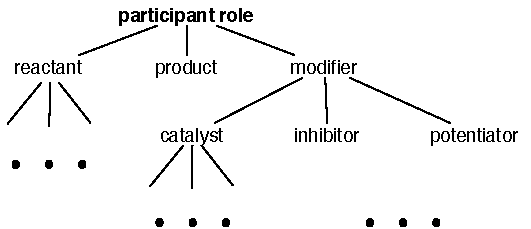
\includegraphics[scale = 0.9]{figs/sbo-participant-role}
  \caption{Partial expansion of some of the terms in the
    \emph{participant role} CV of SBO.}
  \label{fig:expanded-species}
\end{figure}

Figure~\ref{fig:expanded-species} shows the anticipated structure
for the \emph{participant role} CV which reflects the hierarchical
conceptual groupings of the concepts. For example, in reaction
rate expressions, there are a variety of possible modifiers.  Some
classes of modifiers can be further subdivided and grouped.  All
of this is easy to capture in the CV.  As more agreement is
reached in the modeling community about how to define and name
modifiers for different cases, the CV can grow to accommodate it.

\begin{figure}[tbh]
  \vspace*{2ex}
  \centering
  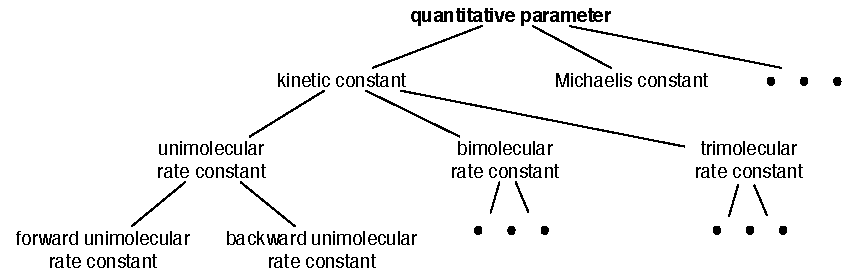
\includegraphics[scale = 0.9]{figs/sbo-quantitative-parameter}
  \caption{Partial expansion of some of the terms in the \emph{quantitative
      parameter} CV.}
  \label{fig:expanded-parameter}
\end{figure}

Similar to the above, the controlled vocabulary for quantitative
parameters also has a hierarchical structure, as illustrated in
Figure~\ref{fig:expanded-parameter}.  Note the separation of
\emph{kinetic constant} into separate terms for unimolecular,
bimolecular, etc. reactions, as well as for for forward and
reverse reactions.  The need to have separate terms for forward
and reverse rate constants arises in reversible mass-action
reactions.  This distinction is not always necessary for all
quantitative parameters; for example, there is no comparable
concept for the Michaelis constant.  Another distinction for some
quantitative parameters is a decomposition into different versions
based on the modeling framework being assumed.  For example,
different terms for continuous and discrete formulations of
kinetic constants represent specializations of the constants for
particular simulation frameworks.  Not all quantitative parameters
will need to be distinguished along this dimension.

\begin{wrapfigure}[6]{r}{2.85in}
%\begin{figure}[h]
  \centering
  \vspace*{-2ex}
  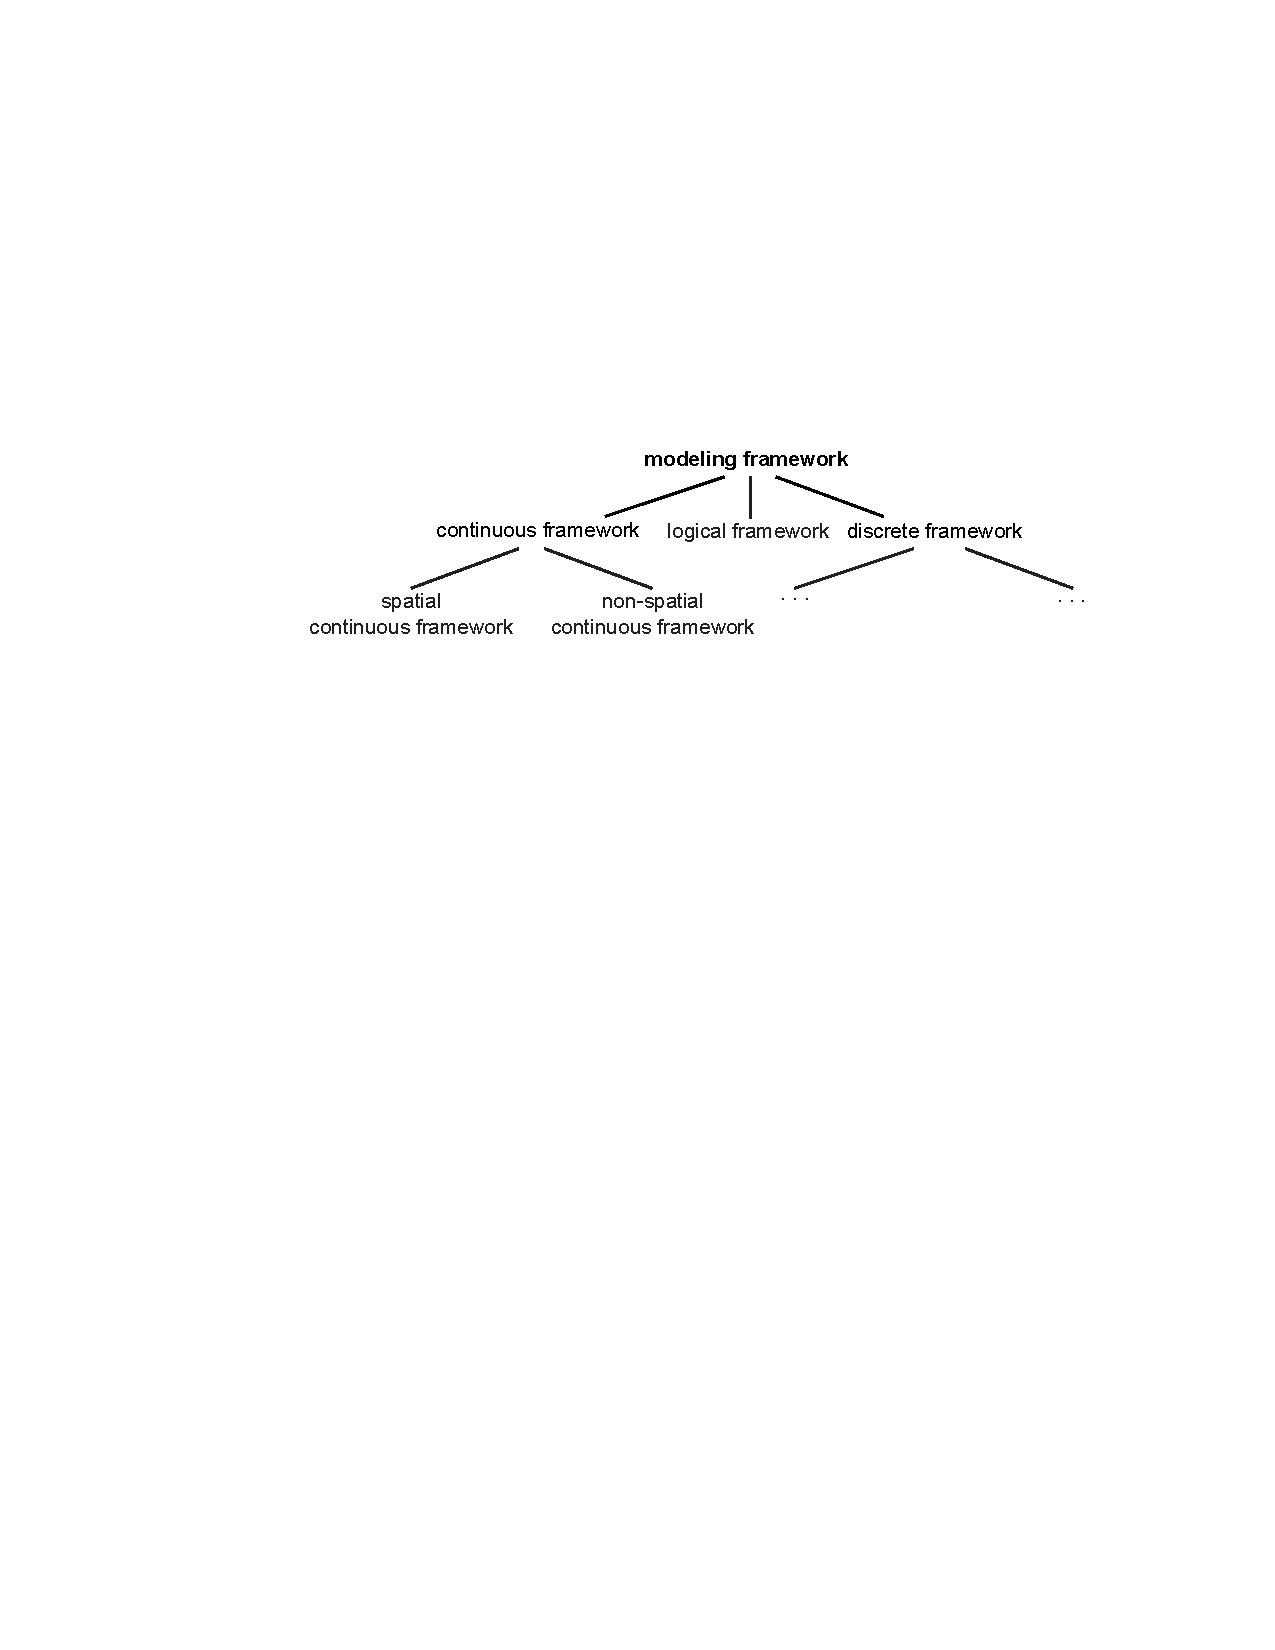
\includegraphics[scale = 0.9]{figs/sbo-framework}
  \vspace*{-2ex}
  \caption{Partial expansion of some of the terms in the
    \emph{modeling framework} CV.}
  \label{fig:expanded-framework}
\end{wrapfigure}
%\end{figure}
The \emph{modeling framework} controlled vocabulary is needed to
support labeling models and reactions with the framework for which
they are designed.  Figure~\ref{fig:expanded-framework}
illustrates the structure of this CV, which is at this point
extremely simple, but we expect that more terms will evolve in the
future.

Finally, there is the \emph{mathematical expression} framework.
This controlled vocabulary encompasses the various mathematical
expressions that constitute a model.
Figure~\ref{fig:sbo-math-expression} illustrates a portion of the
hierarchy.  Rate law formulas are part of the mathematical
expression hierarchy, and subdivided by successively more refined
distinctions until the leaf terms represent precise statements of
common reaction types.  Other types of mathematical expressions
are likely to be included in order to be able to characterize
other mathematical components of a model, namely initial
assignments, assignment rules, rate rules, algebraic rules,
constraints, and event triggers and assignments.

\begin{figure}[tbh]
  \centering
  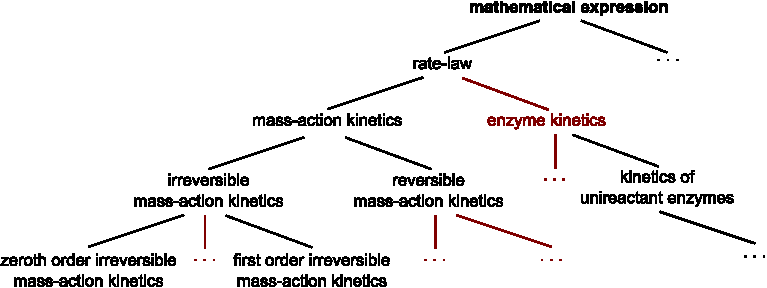
\includegraphics[scale = 0.97]{figs/sbo-math-expression}
  \caption{Partial expansion of some of the terms in the \emph{mathematical
      expression} CV.}
  \label{fig:sbo-math-expression}
\end{figure}

The leaf terms of the rate law portion of the SBO mathematical
expression framework contain the mathematical formulas for the
rate laws encoded using \mathmltwo.  There are many potential uses
for this.  One is to allow a software application to obtain the
formula and insert it into a model.  In effect, the formulas given
in the CV act as templates for what to put into an SBML
\KineticLaw definition.  The MathML definition also acts as a
precise statement about the rate law in question.

To make this discussion concrete, here is an example definition of
an entry in the SBO rate law hierarchy at the time of this
writing.  This term represents second-order, irreversible,
mass-action kinetics with one reactant, formulated for use in a
continuous modeling framework:
\begin{quote}
\begin{description}

\item \emph{ID}: \token{SBO:0000052}

\item \emph{Name}: second order irreversible mass action kinetics,
  one reactant, continuous scheme

\item \emph{Definition}: Reaction scheme where the products are
  created from the reactants and the change of a product quantity
  is proportional to the product of reactant activities. The
  reaction scheme does not include any reverse process that
  creates the reactants from the products, and the change of a
  product quantity is proportional to the square of one reactant
  quantity. It is to be used in a reaction modeled using a
  continuous framework.

\item \emph{Parent(s)}: \token{SBO:0000052}, first-order
  irreversible mass-action kinetics (is a)

\item \emph{MathML}:
\begin{example}
<math xmlns="http://www.w3.org/1998/Math/MathML">
   <lambda>
     <bvar><ci definitionURL="http://biomodels.net/SBO/#SBO:0000036">k</ci></bvar>
     <bvar><ci definitionURL="http://biomodels.net/SBO/#SBO:0000010">R</ci></bvar>
     <apply>
         <times/>
         <ci>k</ci>
         <ci>R</ci>
         <ci>R</ci>
     </apply>
   </lambda>
</math>
\end{example}

\end{description}
\end{quote}

In the MathML definition of the term shown above, the bound
variables in the \token{lambda} expression are tagged with
references to terms in the SBO quantitative parameter (for
\token{k}) and SBO participant role (for \token{R}) vocabularies.
This makes it possible for software applications to interpret the
intended meanings of the parameters in the expression.


%\subsubsection{Interacting with the Systems Biology Ontology}

%We fully anticipate that web service interfaces and software
%libraries will be made available to provide application
%programming interfaces (APIs) to the Systems Biology Ontology,
%allowing software applications to access definitions of SBO terms
%and relationships between them.  The actual SBO ontology is stored
%in a database, but it may be helpful to discuss the content of the
%entries in order to get a sense for the kinds of data fields that
%are likely to be available for each entry in SBO.  The following
%are the minimum anticipated data fields:
%\begin{itemize}\setlength{\parskip}{-0.2ex}

%\item \emph{Identifier}: Each term has a unique identifier of type
%  \primtype{SBOType} (Section~\ref{sec:sboterm-type}).

%\item \emph{Name}: Each term is given a name; \eg ``unimolecular
%  rate constant''.

%\item \emph{Definition}: Each term includes a written description
%  of its intended meaning.  For example, for ``unimolecular rate
%  constant'', this might be ``Numerical parameter that quantifies
%  the velocity of a chemical reaction involving only one
%  reactant.''

%\item \emph{MathML}: For terms that represent final mathematical
%  expressions (\ie the leaf terms of \sbomathformula), the formula
%  is represented using generic \mathmltwo.

%\item \emph{Parents}: The term(s) from which a given term is
%  derived.  The given term has an ``is a'' relationship to its
%  parents.

%\item \emph{Comment}: Additional notable information about the
%  CV term, on an as-needed basis.

%\end{itemize}

%Note that the definitions of formulas, in particular the rate
%laws, are recorded in generic \mathmltwo format.  They
%purposefully do not contain SBML markup.  This permits other,
%non-SBML-aware software applications to use SBO for other
%purposes, and likewise, for other kinds of ontologies to interlink
%with SBO.

One of the goals of SBO is to permit a tool to traverse up and
down the hierarchy in order to find equivalent terms in different
frameworks.  The hope is that when a software tool encounters a
given rate formula in a model, the formula will be a specific form
(say, ``mass-action kinetics, second order, one reactant, for
discrete simulation''), but by virtue of the consistent
organization of the reaction rate CV into framework-specific
definitions, the tool should in principle be able to determine the
definitions for other frameworks (say, ``mass-action kinetics,
second order, one reactant for \emph{continuous} simulation'').
If the software tool is designed for continuous simulation and it
encounters an SBML model with rate laws formulated for discrete
simulation, it could in principle look up the rate laws'
identifiers in the CV and search for alternative definitions
intended for discrete simulation.  And of course, the converse is
true, for when a tool designed for discrete simulation encounters
a model with rate laws formulated for continuous simulation.


\subsubsection{Relationships between individual SBML components and SBO terms}

The availability of \token{sboTerm} fields on various SBML
components is limited to those for which an SBO label is
appropriate given the goals and principles of SBO's use in SBML
(Section~\ref{sec:sbo-principles}).
Table~\ref{tab:sboterm-availability} summarizes the relationship
between SBML components having \token{sboTerm} fields and the
vocabularies within SBO that apply to that component.

% NOTE: make sure the list in this table matches what's
% defined in \sboelements at the top of this file.

\begin{table}[bht]
  \small
  \centering
  \begin{edtable}{tabular}{lll}
    \toprule
    \textbf{SBML Component}   & \textbf{SBO Vocabulary} & \textbf{Parent SBO Identifier} \\
    \midrule
    \Model                    & modeling framework      & \sboframeworkID \\
    \Reaction                 & modeling framework      & \sboframeworkID \\
    \Parameter                & quantitative parameter  & \sboparameterID \\
    \SpeciesReference         & participant role        & \sboparticipantID \\
    \ModifierSpeciesReference & participant role        & \sboparticipantID \\
    \FunctionDefinition       & mathematical expression & \sbomathformulaID \\
    \KineticLaw               & mathematical expression & \sbomathformulaID \\
    \InitialAssignment        & mathematical expression & \sbomathformulaID \\
    \AlgebraicRule            & mathematical expression & \sbomathformulaID \\
    \AssignmentRule           & mathematical expression & \sbomathformulaID \\
    \RateRule                 & mathematical expression & \sbomathformulaID \\
    \Constraint               & mathematical expression & \sbomathformulaID \\
    \Event                    & mathematical expression & \sbomathformulaID \\
    \EventAssignment          & mathematical expression & \sbomathformulaID \\
    \bottomrule
  \end{edtable}
  \caption{SBML components and the main types of SBO terms that
  may be assigned to them.  The parent identifiers are provided
  for guidance, but actual annotations should use more specific
  child terms.  See text for explanation.}
  \label{tab:sboterm-availability}
\end{table}

The parent identifiers shown in
Table~\ref{tab:sboterm-availability} are provided for reference.
They are the highest-level terms in their respective vocabularies;
however, these are \emph{not} the terms that would be used to
annotate an element in SBML, because there are more specific terms
underneath the parents shown here.  A software tool should use the
most specific SBO term available for a given concept rather than
using the top-level identifier acting as the root of that
particular vocabulary.

%\subsubsection{Examples}
%\label{sec:sboterm-examples}

%% FIXME

%\textbf{NEED EXAMPLES}


\subsection{Relationships to the SBML \token{annotation} field}

Another means of providing this kind of information would be to
place it inside the \token{annotation} field
(Sections~\ref{sec:sbase} and~\ref{sec:annotation-standard}).
Although \token{sboTerm} is just another kind of optional
annotation in SBML, the SBO references are separated out and given
a separate field on SBML components, both to simplify their use
for software tools and because they assert a slightly stronger and
more focused connection in a more regimented fashion.  SBO term
references are intended to allow a modeler to make a statement of
the form ``this object is identical in meaning and intention to
the definition of X in the SBO vocabulary'' and do so in a way
that a \emph{software tool can interpret unambiguously}.


\subsubsection{Tradeoffs in using SBO terms}

The SBO-based approach to annotating SBML components with
controlled terms has the following strengths:
\begin{enumerate}

\item The syntax is minimally intrusive and maximally simple,
  requiring only one string-valued attribute.

\item It supports a significant fraction of what SBML users have wanted
  to do with controlled vocabularies.

\item It does not interfere with any other scheme.  The more
  general annotation-based approach described in
  Section~\ref{sec:annotation-standard} can still be used
  simultaneously in the same model.

\end{enumerate}

The scheme has the following weaknesses:
\begin{enumerate}

\item An object can only have one \token{sboTerm} field,
  therefore, it can only be related to a single term in SBO.
  (This also impacts the design of SBO: it must be structured such
  that a class of SBML elements can logically only be associated
  with one class of terms in the ontology.)

\item The only relationship that can be expressed by
  \token{sboTerm} is ``is a''.  It is not possible to represent
  different relationships (known as \emph{verbs} in
  ontology-speak).  This limits what can be expressed.

\end{enumerate}

The weaknesses are not shared by the annotation scheme described
in Section~\ref{sec:annotation-standard}.  If an application's
needs cannot be met using SBO terms, software developers should
examine the approach described in
Section~\ref{sec:annotation-standard}.


\subsubsection{When to use SBO and when to use other annotations}

The general annotation guidelines described in
Section~\ref{sec:annotation-standard} could also be used to make
references to SBO terms.  However, in the interest of making the
use of SBO in SBML maximally interoperable between software tools,
the best-practice recommendation is to place SBO references in the
\token{sboTerm} field rather than in the \token{annotation} field
of an object.

Some software applications may have their own vocabulary of terms
similar in purpose to SBO.  For maximal software interoperability,
the best-practice recommendation in SBML is nonetheless to use SBO
terms in preference to using application-specific annotation
schemes.  Software applications should therefore attempt to
translate their private terms to and from SBO terms when writing
and reading SBML, respectively.


\subsection{Discussion}

Here we discuss some additional points about the SBO-based
approach.

\subsubsection{Frequency of change in the ontology}
\label{sec:sbo-frequency-of-change}

The SBO development approach follows conventional ontology
development approaches in bioinformatics.  One of the principles
being followed is that identifiers and meanings of terms in the
CVs never change and the terms are never deleted.  Where some
terms are deemed obsolete, the introduction of new terms refine or
supersede existing terms, but the existing identifiers are left in
the CV.  Thus, references never end up pointing to nonexistent
entries.  In the case where synonymous terms are merged after
agreement that multiple terms are identical, the term identifiers
are again left in the CV and they still refer to the same concept
as before.  Out-of-date terms cached or hard-coded by an
application remain usable in all cases.  (Also, with
machine-readable CV encodings and appropriate software design, it
should be possible to develop API libraries that automatically map
older terms to newer terms as the CVs evolve.)

Therefore, a model is never in danger of ending up with SBO
identifiers that cannot be dereferenced.  If an application finds
an old model with a term \token{SBO:0000065}, it can be assured
that it will be able to find this term in SBO, even if it has been
superseded by other, more preferred terms.


\subsubsection{Consistency of information}

If you have a means of linking (say) a reaction rate formula to a
term in a CV, is it possible to have an inconsistency between the
formula in the SBML model and the one defined for the CV term?
Yes, but this is not a new problem; it arises in other situations
involving SBML models already.  The guideline for these situations
is that the model must be self-contained and stand on its own.
Therefore, in cases where they differ, the definitions in the SBML
model take precedence over the definitions referenced by the CV.
In other words, the model (and its MathML) is authoritative.


\subsubsection{Implications for network access}
\label{sec:sbo-implications-for-network-access}

Must a software tool have the ability to access the network or
read the CV every time it encounters a model or otherwise works
with SBML?  No.  Since the SBO will likely stabilize and change
infrequently once a core set of terms is defined, applications can
cache the controlled vocabulary and not make network accesses to
the master SBO copy unless something forces them to (\eg detecting
a reference in a model to an SBO term that the application does
not recognize).  In addition, applications could have user
preference settings indicating how often the CV definitions should
be refreshed (similar to how modern applications provide a setting
dictating how often they should check for new versions of
themselves).  Simple applications may go further and hard code
references to terms in SBO that have reached stability and
community consensus.


\subsubsection{Implications for software tools}

What if a software tool does not pay attention to the SBO
annotations described here?  Then one is faced with exactly the
situation that exists today: the SBML model must be interpreted
as-is, without benefit of the information added by the SBO terms.
The purpose of introducing an ontology scheme and guidelines for
its use is to give tools enough information that they \emph{could}
perform added processing, if they were designed to take advantage
of that information.


\subsubsection{Is another ontology really needed?}

It may seem that developing a new, separate ontology is overkill
for the intended purpose.  However, it turns out that no existing
ontology contains the necessary details for this role in SBML.  In
particular, none of the existing ontologies provide mathematical
formulas for reaction rates.
